\documentclass[../main.tex]{subfiles}

\begin{document}

El corazón humano contrae sus músculos mediante pulsos eléctricos, pero en algunos casos estos no son capaces de ser generados regularmente. El continuo progreso de la ciencia ha permitido la creación de dispositivos llamados marcapasos cada vez más avanzados cuya función es generar estos pulsos y así mejorar la salud del corazón del paciente. Los impulsos eléctricos son creados mediante los llamados \textit{circuitos de estímulos}, que no es más que un conjunto de resistencias y condensadores unidos a una fuente de alimentación; o lo que es lo mismo, un circuito RC. \cite{intro_circuitos_RC} \\

Las aplicaciones de este tipo de circuitos no se centran solamente en el área de la medicina, sino que también podemos encontrarlos en objetos de uso cotidiano. Si observamos algunos de los auriculares de última generación que llevan incorporados una serie de funciones que permiten aislar ruido del exterior, vemos que estos utilizan lo que se conoce como \textit{filtros de paso}, que dependiendo de si se quieren escuchar frecuencias altas, bajas o en un rango, se utilizarán respectivamente los filtros de paso alto, bajo o de banda. Estos filtros no son más que circuitos RC dónde sus componentes se encuentran dispuestos de diferente manera según el objetivo que se quiere conseguir. Y, aunque normalmente las frecuencias de filtrado ya vienen configuradas de fábrica, existen modelos en los que estas pueden cambiarse mediante el uso de resistencias variables.\\

Otro uso de estos circuitos serían en las \textit{fuentes de luz estroboscópicas}. Se trata de una fuente de luz cuya emisión se produce de forma intermitente. Este tipo de dispositivos podemos encontrarlos en los \textit{strobes} de un avión (los focos de color rojo y verde que se sitúan en los extremos de las alas y cuya función es posicionar a la aeronave para evitar colisiones) o en cámaras de fotografía para tomar instantáneas de objetos en movimiento, como se puede ver en la figura \ref{foto_estroboscópica}.

\begin{figure}[!h]
          \centering
          \includegraphics[width=0.5\textwidth]{images/foto_estroboscópica.png}
          \caption{Movimiento de un balón usando una \textit{cámara estroboscópica}. \url{https://upload.wikimedia.org/wikipedia/commons/3/3c/Bouncing_ball_strobe_edit.jpg}}
          \label{foto_estroboscópica}
\end{figure}

Por otro lado tenemos los circuitos RL. Un ejemplo de uso de este tipo de circuitos lo encontramos durante el proceso de combustión en un motor de gasolina. Para que esta se lleve a cabo, el combustible debe de mezclarse con una serie de gases inflamables a alta presión y posteriormente, se debe de producir una chispa que queme esta mezcla. Para ello se hace uso de las bujías, unos dispositivos compuestos por dos hilos separados entre sí entre los que se produce una alta diferencia de potencial creando así un arco voltaico que es capaz de iniciar la combustión en el interior del motor. Pero normalmente los vehículos que emplean estos motores suelen ser alimentados por baterías de 12V o 24V, siendo estos voltajes insuficientes para que las bujías puedan llegar a inducir esa chispa.

Además de en motores de combustión de gasolina, este tipo de circuitos podemos hallarlos en dispositivos de filtrado de frecuencia (similares a los construidos con circuitos RC) o en circuitos osciladores. Estos últimos pueden usarse para la construcción de generadores de ondas de radio o televisón y en receptores usados en la telefonía móvil. Estos se encuentran formados por una serie de condensadores, resistencias y bobinas conectadas, también llamados circuitos RLC. Aunque estos sean otro caso de uso de bobinas y condensadores, estos circuitos no son objeto de estudio en este trabajo así que a continuación, nos centraremos en el estudio de los circuitos RC y RL en corriente continua y estado transitorio.


\subsection{El condensador y el circuito RL}
En primer lugar, comenzamos definiendo qué es un condensador. Este se trata de un dispositivo compuesto generalmente por dos placas conductoras aisladas entre sí, a través de un medio vacío, aire o algún material aislante; comunmente llamado diélectrico, en el que podemos almacenar energía eléctrica.\\ 

La cantidad de energía que puede almacenarse en un condensador depende de la relación que existe entre la carga de cada una de las armaduras y de la diferencia de potencial que se aplica entre ellas. A dicha relación se le conoce como \textit{capacidad} y su unidad de medida en el Sistema Internacional(a partir de ahora S.I.) es el \textit{faradio} ($F$); que es equivalente a un culombio ($C$) de carga por cada voltio ($V$) de potencial eléctrico aplicado.

\begin{equation}
    \label{def::capacidad_conductor}
    C = \frac{Q}{V}
\end{equation}

Los conductores más utilizados suelen tener forma cilíndrica, aunque también los hay planos o esféricos. La geometría de estos dispositivos afecta directamente a su capacidad, lo que puede complicar su cálculo si la figura del condensador es demasiado compleja. Así que para simplificar lo máximo posible tanto los cálculos como la posterior implementación de un condensador en la simulación, no tendremos en cuenta la forma del condensador sino que se trabajará directamente con la capacidad del mismo.\\ 

Ya se comentó en la introducción de este capítulo que un circuito RC es una asociación de resistencias eléctricas y condensadores. Es por eso que, como el objetivo que queremos alcanzar es elaborar una simulación que recoja los fundamentos de la carga y descarga del condensador, nos ceñiremos a los circuitos RC de primer orden en corriente continua; es decir, aquellos que cuentan con una resistencia y un condensador conectados en serie alimentados por una pila.\\ 

\begin{figure}[!h]
    \centering
    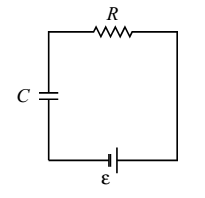
\includegraphics[width=0.3\textwidth]{images/Circuito_RC.png}
    \caption{Representación de un circuito RC de primer orden.}
    \label{fig::circuito_rc_representación}
\end{figure}

Partimos entonces de un condensador de capacidad $C$ completamente descargado conectado en serie a una resistencia de valor $R$. En el instante de tiempo $t=0s$, aplicamos una diferencia de potencial de $\varepsilon V$, cuyo valor coincide con el voltaje característico de la fuente utilizada (figura \ref{fig::circuito_rc_representación}).

En ese mismo instante, la carga del condensador es nula, así que utilizando la definición de capacidad llegamos a la conclusión de que el potencial en él también lo es. Por el contrario, como siempre debe de cumplirse el principio de conservación de la energía; hablando en términos de potencial eléctrico, el voltaje entre los bornes de la resistencia debe de ser máximo, por lo que la intensidad de corriente que circula en ese momento por el circuito también lo es. 

A medida que el condensador va ganando carga y el potencial eléctrico entre sus placas aumenta, sabiendo que la fuerza electromotriz de la fuente es constante y que debe de cumplirse el principio de conservación energético, el potencial en la resistencia disminuye. Esto se debe a que estos circuitos son estacionarios; es decir, las magnitudes que lo describen varían a lo largo del tiempo.

\begin{figure}[!h]
    \centering
    \subfloat[$t = 0s$]{
        \label{fig::circuito_rc2}
        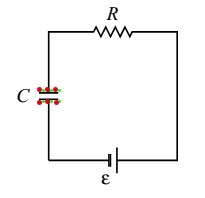
\includegraphics[width=0.33\textwidth]{images/Circuito_RC_2.png}
    }
    \subfloat[Proceso de carga.]{
        \label{fig::circuito_rc3}
        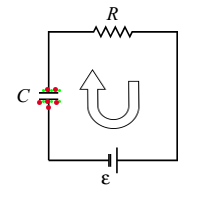
\includegraphics[width=0.33\textwidth]{images/Circuito_RC_3.png}
    }
    \subfloat[Carga completa]{
        \label{fig::circuito_rc4}
        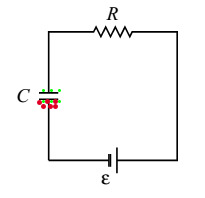
\includegraphics[width=0.33\textwidth]{images/Circuito_RC_4.png}
    }
    \caption{Fases del estado de carga de un condensador. Los puntos rojos hacen referencia a los electrones en movimiento.}
    \label{fig::carga_condensador}
\end{figure}

Así que para observar con más detalle como evolucionan cada una de las magnitudes basta con realizar un balance energético en términos de potencial, dónde la energía suministrada por la fuente debe de ser en todo momento igual a la consumida por los componentes pasivos del circuito: el condensador y la resistencia.


\begin{equation}
    \varepsilon = V_C(t) + V_R(t) = \frac{q(t)}{C} + R\frac{\partial q(t)}{\partial t}
    \label{eqq::balance_energetico_rc_1}
\end{equation}

En este caso, tenemos que $\varepsilon$ es la fuerza electromotriz de la fuente (o la energía suministrada por la pila por cada unidad de carga que la atraviesa), $V_C(t)$ hace referencia al potencial eléctrico entre las armaduras del condensador y $V_R(t)$ a la diferencia de potencial en la resistencia. Resolviendo la ecuación diferencial ordinaria anterior, obtenemos las expresiones que modelan la carga del condensador que se muestran en la tabla \ref{tab::ecuaciones_carga_rc}.


\begin{table}[!ht]
    \begin{center}
        \begin{tabular}{|| c | c | c ||}
            \hline
            \textbf{Concepto} & \textbf{Expresión} &  \textbf{Resolución}\\ \hline
            Carga del condensador & $q(t) = C\varepsilon \left( 1 - e^{\frac{-t}{RC}} \right)$ & \ref{part::carga_condensador_1} \\
            Intensidad de corriente & $I(t) = \frac{\varepsilon}{R}e^{\frac{-t}{RC}}$ & \ref{part::carga_condensador_2} \\
            Diferencia de potencial resistencia & $V_R(t) = \varepsilon \cdot e^{\frac{-t}{RC}}$ & \ref{part::carga_condensador_3} \\ 
            Diferencia de potencial condensador & $V_C(t) = \varepsilon \left(1- e^{\frac{-t}{RC}}\right)$ & \ref{part::carga_condensador_4} \\ 
            Energía del condensador & $E(t) = \frac{1}{2}CV_C(t)^2 $ & \ref{part::energia_condensador}
            \\
            \hline
            \end{tabular}
            \caption{Modelado del estado de carga del condensador.}
            \label{tab::ecuaciones_carga_rc}
    \end{center}
\end{table}





\subsection{El condensador y el circuito RC}




    
Con esto ya conocemos cuáles son las expresiones que se encargan de modelar la carga del condensador y que utilizaremos posteriormente cuando hagamos la implementación de este apartado de la simulacion del circuito RC. \\


Continuamos entonces con el modelado de la descarga del condensador. Antes de dar comienzo a la descarga, supondremos que estamos en la situación descrita por la figura \ref{fig::circuito_rc4}. Partimos entonces de un condensador completamente cargado, cuyo valor de carga denotaremos por $q_{max}$; y que además los valores de la diferencia de potencial en los terminales del dispositivo ($V_L$) y de la energía almacenada ($E$) en él son máximos. Puesto que no se está produciendo movimiento de cargas, la intensidad de corriente es nula, al igual que la diferencia de potencial en la resistencia. \\

\begin{figure}[!h]
    \centering
    \subfloat[Condensador cargado]{
        \label{fig::circuito_rc5}
        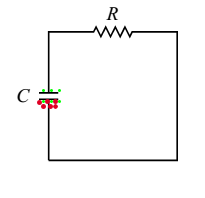
\includegraphics[width=0.33\textwidth]{images/Circuito_RC_5.png}
    }
    \subfloat[Movimiento de cargas eléctricas]{
        \label{fig::circuito_rc6}
        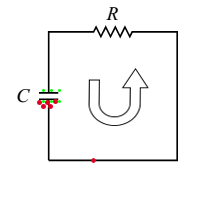
\includegraphics[width=0.33\textwidth]{images/Circuito_RC_6.png}
    }
    \subfloat[Descarga completada]{
        \label{fig::circuito_rc7}
        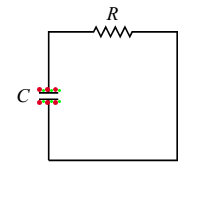
\includegraphics[width=0.33\textwidth]{images/Circuito_RC_7.png}
    }
    \caption{Fases del estado de descarga de un condensador}
    \label{fig::descarga_condensador}
\end{figure}

Así que para descargar el condensador, debemos de quitar del circuito la fuente de alimentación. Sin energía que suministrar, las cargas de la placa negativa del condensador se verán atraídas por las cargas de la placa positiva, produciendo así un movimiento de electrones que inducirán corriente eléctrica en sentido contrario a como lo hacían anteriormente. El número de cargas en movimiento disminuirá con el tiempo, produciendo así una caída de tensión en los bornes del condensador y por consiguiente, la pérdida de energía, tal y como se puede ver en la figura \ref{fig::descarga_condensador}. Al final de este proceso el condensador volverá a estar en equilibrio electroestático. \\

Al igual que en el estado de carga, volvemos a realizar un balance energético. En este caso como no disponemos de una fuente de energía, entonces el valor de $\varepsilon$ será cero. Así que planteamos la siguiente ecuación:
\begin{equation}
    0 = V_C(t) + V_R(t)
    \label{eqq::balance_energetico_rc_2}
\end{equation}

, que si resolvemos de forma similar a la anterior, llegamos a obtener las siguientes expresiones que modelan la descarga del condensador (tabla \ref{tab::ecuaciones_descarga_rc}).\\

\begin{table}[!ht]
        \begin{center}
            \begin{tabular}{|| c | c | c ||}
                \hline
                \textbf{Concepto} & \textbf{Expresión} &  \textbf{Resolución}\\ \hline
                Carga del condensador & $q(t) = q_{max} e^{-t/{RC}}$ & \ref{part::descarga_condensador_1} \\
                Intensidad de corriente & $I(t) = \frac{-\varepsilon}{R}e^{\frac{-t}{RC}}$ & \ref{part::descarga_condensador_2} \\
                Diferencia de potencial resistencia & $V_R(t) = -\varepsilon \cdot e^{\frac{-t}{RC}}$ & \ref{part::descarga_condensador_3} \\ 
                Diferencia de potencial condensador & $V_C(t) = \varepsilon   e^{\frac{-t}{RC}}$ & \ref{part::descarga_condensador_4} \\ 
                Energía del condensador & $E(t) = \frac{1}{2}CV_C(t)^2 $ & \ref{part::energia_condensador} \\
                \hline
                \end{tabular}
                \caption{Expresiones que modelan la descarga del condensador}
                \label{tab::ecuaciones_descarga_rc}
        \end{center}
    \end{table}
    
Si estudiamos las expresiones matemáticas de cada una de las magnitudes físicas del circuito, observamos que todas ellas dependen del tiempo ($t$). Además, este tiempo se ve afectado por un valor constante que viene dado por el producto de la capacidad del condensador y del valor óhmico de la resistencia. Definimos a este valor como la \textit{constante de tiempo RC}. Este indica la velocidad de reacción del circuito y que, cuanto mayor sea el valor de esta constante, antes se consigue el estado de equilibrio del mismo. O lo que es lo mismo, el circuito RC de primer orden estudiado se encuentra en estado transitorio, pues los valores de las diferentes magnitudes varían desde un estado inicial a otro final.

\begin{equation}
    \tau_{RC} = R \cdot C
    \label{eqq::constante_tiempo_rc}
\end{equation}

Para comprobar que efectivamente el comportamiento de cada una de las magnitudes es el esperado, vamos a analizar los resultados de un circuito de ejemplo, tomando una fuente con un voltaje de $\varepsilon=12V$, una resistencia con valor óhmico de $R=1000\Omega$ y un condensador con una capacidad de $C=10 \mu F$. Calcularemos los valores de cada una de las magnitudes físicas hasta un tiempo de $t=5 \cdot \tau_{RC}$ segundos, el cuál debería de ser suficiente para comprender qué esta ocurriendo en cada caso.

Analizamos entonces los resultados obtenidos (figura \ref{fig::circuito_rc_simulacion_results}). En primer lugar, cuando el circuito se encuentra dispuesto para la carga del condensador, podemos observar que a medida que transcurre el tiempo, la carga de este dispositivo aumenta y, por consiguiente, lo hacen el potencial y la energía almacenada en el mismo. El número de cargas negativas que pueden moverse a una placa del condensador a la otra será cada vez menor, así que la intensidad de corriente que circula por el circuito irá disminuyendo hasta ser cero. De la misma forma, el potencial de la resistencia también caerá hasta ser nulo. 

Para la descarga del condensador, el movimiento de las cargas es en sentido contrario (se mueven de la placa cargada negativamente, hasta la cargada positivamente). Esto impulsa un movimiento de cargas negativas por lo que aparece una intensidad de corriente. El condensador actúa como una fuente de alimentación, así que las cargas que se desplazan de una placa a otra hacen que la carga de este dispositivo disminuya junto al potencial entre sus terminales y la energía almacenada. Como el número de cargas es cada vez menor, ocurre igual que en el estado anterior: tanto la intensidad de corriente como el potencial en la resistencia disminuirán con el tiempo.\\


\begin{figure}[!h]
    \centering
    \captionsetup[subfloat]{labelformat=empty}
        \subfloat[]{
        
            \resizebox{0.45\textwidth}{!}{
        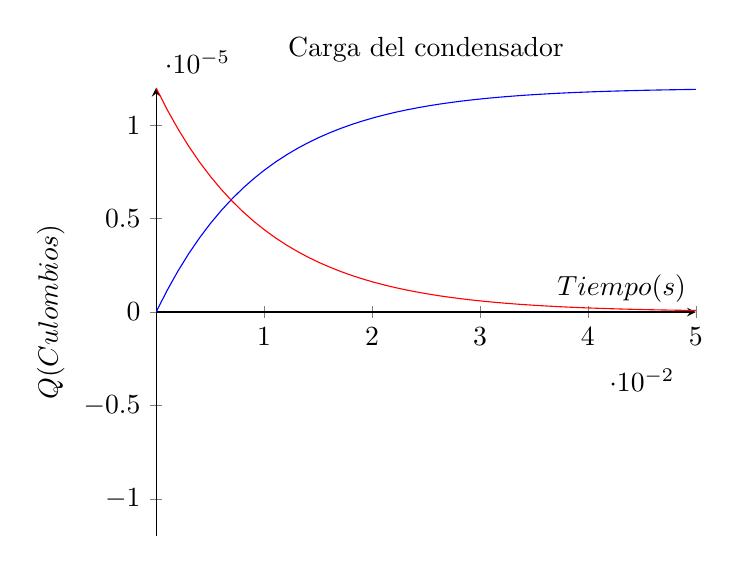
\begin{tikzpicture}
            \begin{axis}[
                title={Carga del condensador},
                axis y line = left,
                axis x line = middle,
                xmin=0, xmax=0.05,
                ymin=-0.000012, 
                xlabel = \(Tiempo (s)\),
                ylabel = {\(Q (Culombios)\)},
            ]
            %Below the red parabola is defined
            \addplot [
                domain=0:0.1, 
                samples=100, 
                color=blue,
            ]
            {0.000012*(1-exp(-x/0.01))};
             
            \addplot [
                domain=0:0.1, 
                samples=100, 
                color=red,
            ]
            {0.000012*exp(-x/0.01)};
        
        \end{axis}
        \end{tikzpicture}
        }
        \resizebox{0.45\textwidth}{!}{
        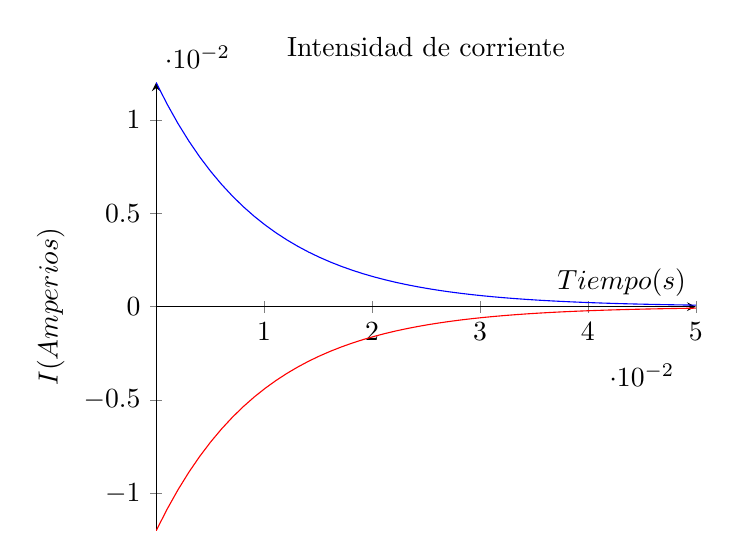
\begin{tikzpicture}
            \begin{axis}[
                title={Intensidad de corriente},
                axis y line = left,
                axis x line = middle,
                xmin=0, xmax=0.05,
                ymin=-0.012, 
                xlabel = \(Tiempo (s)\),
                ylabel = {\(I (Amperios)\)},
            ]
            %Below the red parabola is defined
            \addplot [
                domain=0:0.1, 
                samples=100, 
                color=blue,
            ]
            {0.012*exp(-x/0.01)};
            
            \addplot [
                domain=0:0.1, 
                samples=100, 
                color=red,
            ]
            {(-0.012)*(exp(-x/0.01))};
        
        \end{axis}
        \end{tikzpicture}
        }
        }
        
        \subfloat[]{
            \resizebox{0.45\textwidth}{!}{
        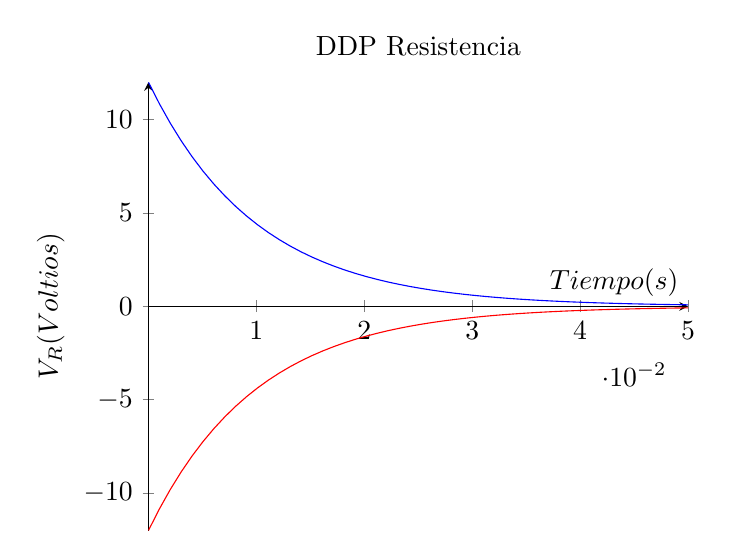
\begin{tikzpicture}
            \begin{axis}[
                title={DDP Resistencia},
                axis y line = left,
                axis x line = middle,
                xmin=0, xmax=0.05,
                ymin=-12, 
                xlabel = \(Tiempo (s)\),
                ylabel = {\(V_R (Voltios)\)},
            ]
            %Below the red parabola is defined
            \addplot [
                domain=0:0.1, 
                samples=100, 
                color=blue,
            ]
            {12*exp(-x/0.01)};
            
            \addplot [
                domain=0:0.1, 
                samples=100, 
                color=red,
            ]
            {-12*exp(-x/0.01)};;
        
        \end{axis}
        \end{tikzpicture}
        }
        \resizebox{0.45\textwidth}{!}{
        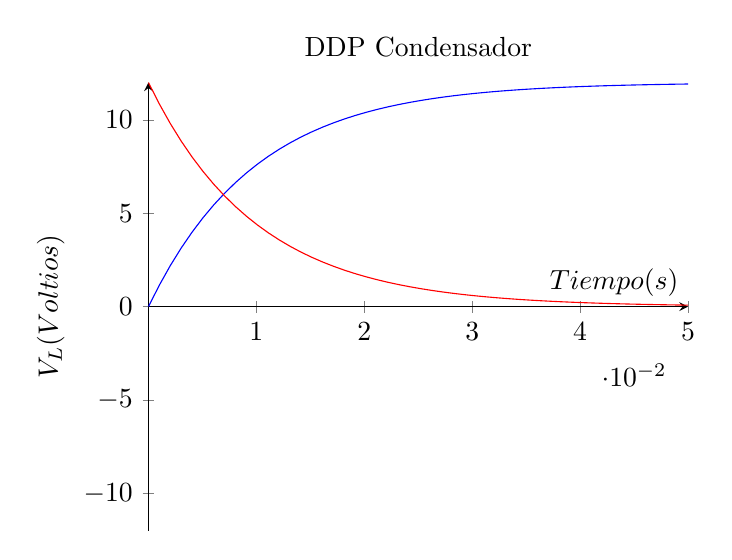
\begin{tikzpicture}
            \begin{axis}[
                title={DDP Condensador},
                axis y line = left,
                axis x line = middle,
                xmin=0, xmax=0.05,
                ymin=-12, 
                xlabel = \(Tiempo (s)\),
                ylabel = {\(V_L (Voltios)\)},
            ]
            %Below the red parabola is defined
            \addplot [
                domain=0:0.1, 
                samples=100, 
                color=blue,
            ]
            {12*(1-exp(-x/0.01))};
            
            \addplot [
                domain=0:0.1, 
                samples=100, 
                color=red,
            ]
            {12*(exp(-x/0.01))};
        
        \end{axis}
        \end{tikzpicture}
        }
        }
        
        \subfloat[]{
            \resizebox{0.45\textwidth}{!}{
        \begin{tikzpicture}
            \begin{axis}[
                title={Energía},
                axis lines = left,
                xmin=0, xmax=0.05,
                ymin=0, 
                xlabel = \(Tiempo (s)\),
                ylabel = {\(E (Julios)\)},
            ]
            %Below the red parabola is defined
            \addplot [
                domain=0:0.1, 
                samples=100, 
                color=blue,
            ]
            {(1/2)*0.00001*(12*(1-exp(-x/0.01)))^2};
            
            \addplot [
                domain=0:0.1, 
                samples=100, 
                color=red,
            ]
            {(1/2)*0.00001*(12*(exp(-x/0.01)))^2};
        
        \end{axis}
        \end{tikzpicture}
        }
        }
    \caption{Evolución de las diferentes magnitudes del circuito RC de ejemplo. En \textit{azul} se muestran los resultados en el estado de carga y en \textit{rojo}, los de descarga.}
    \label{fig::circuito_rc_simulacion_results}
\end{figure}


\subsection{El inductor y el circuito RL}
Como hemos visto en las diferentes aplicaciones durante la introducción de este capítulo, podemos hacer uso de los circuitos RL para incrementar la intensidad de corriente y así, conseguir por ejemplo, aumentar la tensión y crear un arco voltaico con la energía suficiente para quemar combustible en el interior de un motor de gasolina. Para ello utilizamos la \textbf{bobina}, un dispositivo formado principalmente por un hilo conductor enrollado alrededor de un núcleo, normalmente de aire o de algún material ferruginoso (como el hierro o la ferrita).\\


Supongamos entonces que tenemos una bobina y provocamos una intensidad de corriente eléctrica utilizando cualquier fuente de energía, como una pila. Esta variación de corriente (que inicialmente supondremos nula) produce una perturbación en el espacio que es conocida como \textit{campo magnético}, y que por sus propiedades, afecta a todos los objetos con una naturaleza similar; que en este caso, son las cargas en movimiento de dicha corriente eléctrica.


\begin{figure}[!h]
    \centering
    \subfloat[Bobina toroidal con núcleo férrico]{
        \label{fig::bobina_toroidal}
        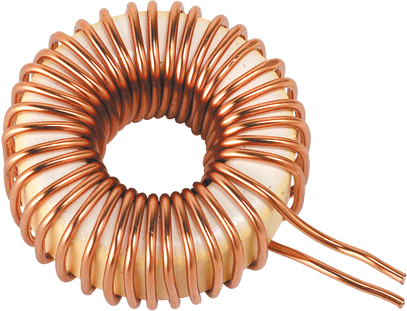
\includegraphics[width=0.33\textwidth]{images/bobina_toroidal.png}
    }
    \subfloat[Bobina espiral con núcleo de aire]{
        \label{fig::bobina_espiral}
        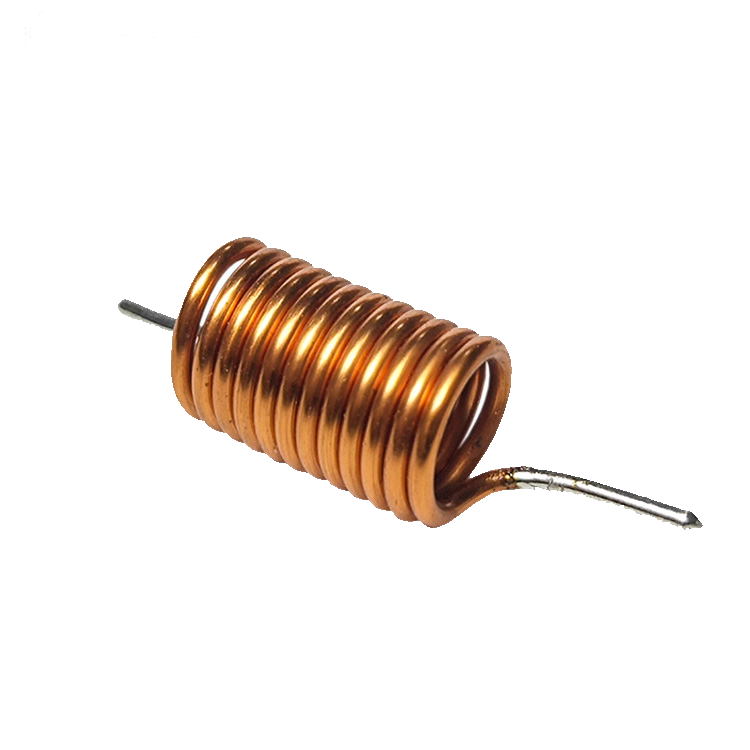
\includegraphics[width=0.33\textwidth]{images/bobina_espiral.png}
    }
    \caption{Tipos de bobinas}
    \label{fig::tipos_bobinas}
\end{figure}

Puesto que la intensidad de corriente ha cambiado, el campo magnético creado por este movimiento de cargas también se ve afectado y como consecuencia, volverá a alterar el valor de la intensidad. A esto se le conoce como el \textbf{fenómeno de autoinducción}, produciendo en la bobina una \textit{F.E.M autoinducida} cuyo valor es directamente proporcional a la variación de \textit{flujo magnético}\footnote{El flujo magnético es la cantidad de campo magnético que atraviesa una superficie, es nuestro caso, la bobina}. A esta magnitud que relaciona intensidad de corriente y flujo magnético recibe el nombre de \textit{coeficiente de autoinducción}, cuyo valor depende exclusivamente del medio dónde la bobina esté sumergida y de su geometría, siendo la unidad de medida en el Sistema Internacional el \textit{henrio} ($H$). Pero al igual que ocurría con el caso de los condensadores, para simplificar los cálculos no vamos a tener en cuenta ni la geometría del inductor ni el medio donde se encuentre, sino que directamente usaremos el coeficiente de autoinducción asociado. \\

\begin{figure}[!h]
          \centering
          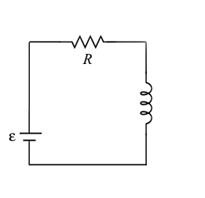
\includegraphics[width=0.3\textwidth]{images/Circuito_RL.png}
          \caption{Representación de un circuito RL de primer orden.}
          \label{fig::circuito_rL_representación}
\end{figure}

Ya sabiendo qué es una bobina, un circuito RL es un conjunto de resistencias eléctricas y bobinas conectadas a una fuente de alimentación. El principal objetivo es comprender la evolución de las diferentes magnitudes físicas que afectan al circuito al inducir corriente eléctrica con estos dispositivos; así que en lugar de analizar un circuito complejo, el análisis y la simulación del mismo se realizará sobre un circuito RL de primer orden. Esto es, un circuito formado por una resistencia y una bobina conectadas en serie. \\

Partimos entonces de un circuito RL de primer orden, donde inicialmente supondremos que la intensidad de corriente que circula por él es nula. En el momento en el que aplicamos una diferencia de potencial al circuito utilizando una fuente de alimentación con un \textit{voltaje característico} de valor $\varepsilon$, se produce una emisión de cargas negativas desde el terminal con carga negativa de la pila. Estas cargas provocan la aparición de un campo magnético en la bobina cuando es atravesada por esta corriente eléctrica, el cuál se ve alterado por el \textit{fenómeno de autoinducción} provocando así un incremento en la intensidad de corriente. Estas cargas en movimiento son impulsadas a través del hilo conductor hasta la placa con carga positiva de la pila; que para mantener el mismo potencial eléctrico entre sus terminales, se origina en su interior una sucesión de reacciones químicas para equiparar esta carga, impulsando cargas negativas desde el cátodo hacia el ánodo de la pila.

\begin{figure}[!h]
    \centering
    \subfloat[Instante inicial. Intensidad nula.]{
        \label{fig::circuito_rl_1 }
        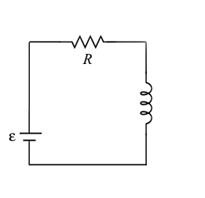
\includegraphics[width=0.33\textwidth]{images/Circuito_RL.png}
    }
    \subfloat[Autoinducción de corriente (carga)]{
        \label{fig::circuito_rl_2}
        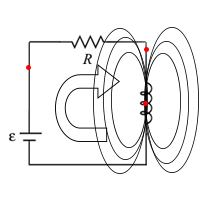
\includegraphics[width=0.33\textwidth]{images/Circuito_RL_2.png}
    }
    \caption{Almacenamiento de energía en una bobina}
    \label{fig::carga_bobina}
\end{figure}

Por supuesto, el \textit{principio de conservación de la energía} debe de cumplirse. Si bien el potencial en los bornes de la bobina disminuye a medida que se incrementa la intensidad de corriente, la diferencia de potencial en la resistencia aumenta. Cuando esta ddp en la resistencia se iguale al valor de la fuente $\varepsilon$, la intensidad del circuito será máxima y por lo tanto, la energía almacenada en el inductor en forma de campo magnético también lo es.

Obtenemos entonces las expresiones matemáticas del modelo realizando un balance energético del circuito, teniendo en cuenta la conservación de la energía en el mismo,

\begin{equation}
    \label{eqq::carga_bobina}
    \varepsilon = V_L(t) + V_R(t)
\end{equation}
, dónde $V_L(t)$ es la diferencia de potencial en el inductor y $V_R(t)$ en la resistencia. De esta ecuación, podemos deducir las expresiones que se muestran en la tabla \ref{tab::ecuaciones_carga_rl}.\\

\begin{table}[!ht]
        \begin{center}
            \begin{tabular}{|| c | c | c ||}
                \hline
                \textbf{Concepto} & \textbf{Expresión} &  \textbf{Resolución}\\ \hline
                Intensidad de corriente & $I(t) = \frac{\varepsilon}{R} \left( 1 - e^{\frac{-Rt}{L}}\right)$ & \ref{part::carga_inductor_1}\\
                Diferencia de potencial resistencia & $V_R(t) = \varepsilon \left( 1 - e^{\frac{-Rt}{L}}\right)$ & \ref{part::carga_inductor_2} \\ 
                Diferencia de potencial inductor & $V_L(t) = \varepsilon   e^{\frac{-Rt}{L}}$ & \ref{part::carga_inductor_3} \\ 
                Energía del inductor & $E(t) = \frac{1}{2}LI(t)^2 $ & \ref{part::energía_inductor} \\
                Flujo magnético & $\phi (t) = L \cdot I(t)$ & \ref{part::flujo_magnetico_inductor} \\
                \hline
                \end{tabular}
                \caption{Expresiones que modelan la carga de la bobina}
                \label{tab::ecuaciones_carga_rl}
        \end{center}
    \end{table}
    
Continuamos entonces con el modelado de la descarga de la bobina. Inicialmente estaremos en el estado descrito por la figura \ref{fig::circuito_rl_2}, cuando la intensidad de corriente que circula por el circuito es máxima. El proceso de disipación de la energía almacenada en el campo magnético de la bobina comienza cuando dejamos de suministrar energía con la fuente de alimentación, es decir, cuando $\varepsilon = 0$ (figura \ref{fig::circuito_rl_3}). \\
    

 \begin{figure}[!h]
    \centering
    \subfloat[Instante inicial. Intensidad máxima.]{
        \label{fig::circuito_rl_3}
        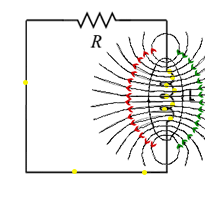
\includegraphics[width=0.33\textwidth]{images/Circuito_RL_3.png}
    }
    \subfloat[Intensidad nula.]{
        \label{fig::circuito_rl_4}
        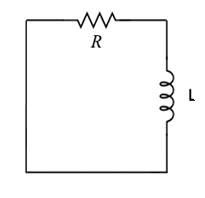
\includegraphics[width=0.33\textwidth]{images/Circuito_RL_4.png}
    }
    \caption{Disipación de energía en una bobina}
    \label{fig::carga_bobina}
\end{figure}

Toda la energía cinética de las cargas en movimiento se disipan en forma de calor cuando estas chocan con las paredes del conductor (a este efecto se le conoce como \textit{efecto Joule}), disminuyendo así la intensidad de corriente hasta ser cero. Puesto que la intensidad ha sufrido una variación respecto a su valor inicial, el campo magnético sufre variaciones (de nuevo por el fenómeno de autoinducción). Además, conforme la intensidad disminuye también lo hacen las tensiones de la resistencia y el inductor, y con ellos la energía almacenada y el flujo magnético de la bobina. Realizando un nuevo balance energético del circuito, obtenemos la siguiente ecuación a resolver, 
\begin{equation}
    \label{eqq::descarga_bobina}
    0 = V_L(t) + V_R(t)
\end{equation}
, a partir de la cuál podemos deducir las expresiones que modelan el comportamiento de cada una de las magnitudes físicas que afectan al circuito durante la descarga de la bobina, tal y como se muestran en la tabla \ref{tab::ecuaciones_descarga_rl}.\\

\begin{table}[!ht]
        \begin{center}
            \begin{tabular}{|| c | c | c ||}
                \hline
                \textbf{Concepto} & \textbf{Expresión} &  \textbf{Resolución}\\ \hline
                Intensidad de corriente & $I(t) = \frac{\varepsilon}{R}  e^{\frac{-Rt}{L}}$ & \ref{part::descarga_inductor1}\\
                Diferencia de potencial resistencia & $V_R(t) = \varepsilon  e^{\frac{-Rt}{L}}$ & \ref{part::descarga_inductor_2} \\ 
                Diferencia de potencial inductor & $V_L(t) = - \varepsilon   e^{\frac{-Rt}{L}}$ & \ref{part::descarga_inductor_3} \\ 
                Energía del inductor & $E(t) = \frac{1}{2}LI(t)^2 $ & \ref{part::energía_inductor} \\
                Flujo magnético & $\phi (t) = L \cdot I(t)$ & \ref{part::flujo_magnetico_inductor} \\
                \hline
                \end{tabular}
                \caption{Expresiones que modelan la descarga de la bobina}
                \label{tab::ecuaciones_descarga_rl}
        \end{center}
    \end{table}

Como podemos observar en todas las expresiones que modelan el circuito RL, todas las magnitudes físicas estudiadas depen del del tiempo ($t$). Este se encuentra afectado por un valor constante que depende del coeficiente de autoinducción y del valor óhmico de la resistencia, al cuál llamaremos \textit{constante de tiempo RL}. Este indica la velocidad de reacción del circuito, y cuanto mayor sea este valor antes se alcanza el estado de equilibrio del circuito. Denotamos a esta constante con el símbolo $\tau_{RL}$. Decimos entonces que este circuito RL se encuentra en estado transitorio; es decir, cada una de las propiedades físicas que lo definen varían desde el estado inicial al final.

\begin{equation}
    \label{eqq::constante_tiempo_rl}
    \tau_{RL} = \frac{L}{R}
\end{equation}

% REVISAR
Para comprobar entonces que el comportamiento de cada una de las magnitudes físicas es el esperado, analizaremos el siguiente circuito de ejemplo. Tomamos una fuente con un voltaje $\varepsilon=12V$, una resistencia de valor óhmico de $R=10 \Omega$ y una bobina con un coeficiente de autoinducción con valor $L=10H$. Calculamos los valores para cada una de estas magnitudes en una simulación con una duración de $t=5\cdot \tau_{RL}$ segundos, que debería de ser suficiente para ver la evolución de cada una de ellas. \\

\begin{figure}[!h]
    \centering
    \captionsetup[subfloat]{labelformat=empty}
        \subfloat[]{
        
            \resizebox{0.45\textwidth}{!}{
        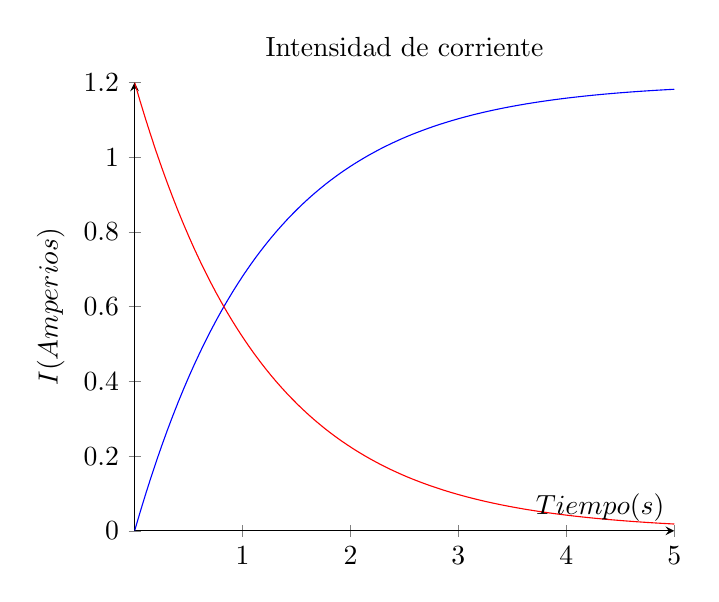
\begin{tikzpicture}
            \begin{axis}[
                title={Intensidad de corriente},
                axis y line = left,
                axis x line = middle,
                xmin=0, xmax=5,
                ymin=-0.000012, 
                xlabel = \(Tiempo (s)\),
                ylabel = {\(I (Amperios)\)},
            ]
            %Below the red parabola is defined
            \addplot [
                domain=0:5, 
                samples=100, 
                color=blue,
            ]
            {1.2*(1-exp(-x*0.838383))};
             
            \addplot [
                domain=0:05, 
                samples=100, 
                color=red,
            ]
            {1.2*(exp(-x*0.838383))};
        
        \end{axis}
        \end{tikzpicture}
        }
        \resizebox{0.45\textwidth}{!}{
        \begin{tikzpicture}
            \begin{axis}[
                title={Energía},
                axis y line = left,
                axis x line = middle,
                xmin=0, xmax=5,
                ymin=-0.012, 
                xlabel = \(Tiempo (s)\),
                ylabel = {\(E (Julios)\)},
            ]
            %Below the red parabola is defined
            \addplot [
                domain=0:5, 
                samples=100, 
                color=blue,
            ]
            {(1/2)*10*(1.2*(1-exp(-x*0.838383)))^2};
            
            \addplot [
                domain=0:5, 
                samples=100, 
                color=red,
            ]
            {(1/2)*10*(1.2*(exp(-x*0.838383)))^2};
        
        \end{axis}
        \end{tikzpicture}
        }
        }
        
        \subfloat[]{
            \resizebox{0.45\textwidth}{!}{
        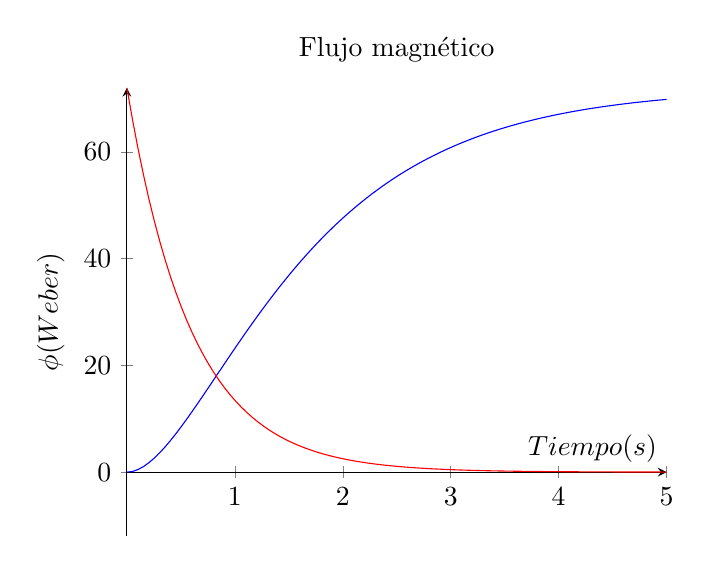
\begin{tikzpicture}
            \begin{axis}[
                title={Flujo magnético},
                axis y line = left,
                axis x line = middle,
                xmin=0, xmax=5,
                ymin=-12, 
                xlabel = \(Tiempo (s)\),
                ylabel = {\(\phi (Weber)\)},
            ]
            %Below the red parabola is defined
            \addplot [
                domain=0:5, 
                samples=100, 
                color=blue,
            ]
            {10*(1/2)*10*(1.2*(1-exp(-x*0.838383)))^2};
            
            \addplot [
                domain=0:5, 
                samples=100, 
                color=red,
            ]
            {10*(1/2)*10*(1.2*(exp(-x*0.838383)))^2};
        
        \end{axis}
        \end{tikzpicture}
        }
        \resizebox{0.45\textwidth}{!}{
        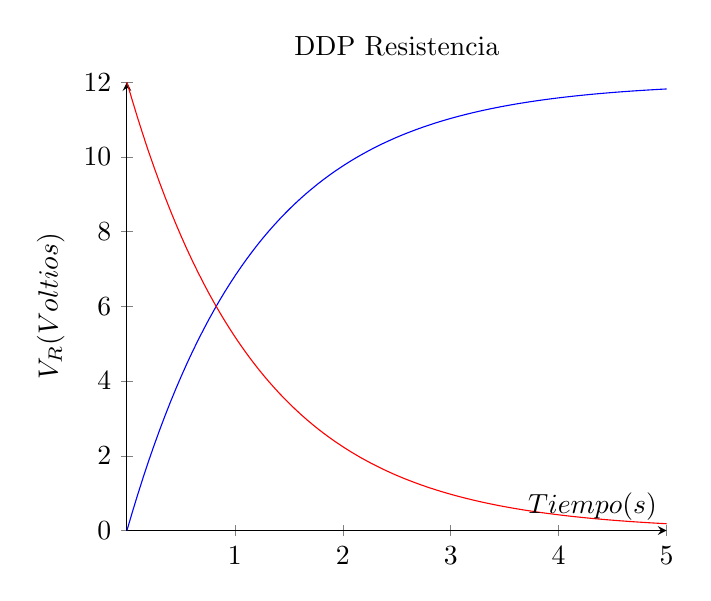
\begin{tikzpicture}
            \begin{axis}[
                title={DDP Resistencia},
                axis y line = left,
                axis x line = middle,
                xmin=0, xmax=5,
                ymin=0, 
                xlabel = \(Tiempo (s)\),
                ylabel = {\(V_R (Voltios)\)},
            ]
            %Below the red parabola is defined
            \addplot [
                domain=0:5, 
                samples=100, 
                color=blue,
            ]
            {12*(1-exp(-x*0.838383))};
            
            \addplot [
                domain=0:5, 
                samples=100, 
                color=red,
            ]
            {12*(exp(-x*0.838383))};
        
        \end{axis}
        \end{tikzpicture}
        }
        }
        
        \subfloat[]{
            \resizebox{0.45\textwidth}{!}{
        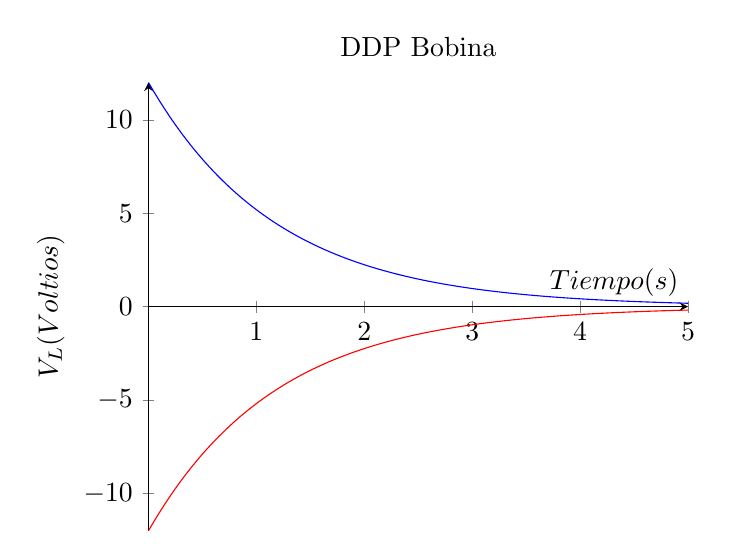
\begin{tikzpicture}
            \begin{axis}[
                title={DDP Bobina},
                axis y line = left,
                axis x line = middle,
                xmin=0, xmax=5,
                ymin=-12, ymax=12,
                xlabel = \(Tiempo (s)\),
                ylabel = {\(V_L (Voltios)\)},
            ]
            %Below the red parabola is defined
            \addplot [
                domain=0:5, 
                samples=100, 
                color=blue,
            ]
            {12*exp(-x*0.838383)};
            
            \addplot [
                domain=0:5, 
                samples=100, 
                color=red,
            ]
            {-12*exp(-x*0.838383)};
        
        \end{axis}
        \end{tikzpicture}
        }
        }
    \caption{Evolución de las diferentes magnitudes del circuito RL de ejemplo. En \textit{azul} se muestran los resultados en el estado de carga y en \textit{rojo}, los de descarga.}
    \label{fig::circuito_rl_simulacion_results}
\end{figure}

Analizamos entonces los resultados de la simulación reflejados en la figura \ref{fig::circuito_rl_simulacion_results}. Cuando la bobina se encuentra en estado de almacenamiento de energía, debido al \textit{fenómeno de autoinducción} anteriormente explicado, tanto la intensidad de corriente como la cantidad de campo magnético (o \textit{flujo magnético}) aumentan; y por consiguiente, lo hacen la energía almacenada en este dispositivo así como la diferencia de potencial en la resistencia. Esta última como se puede ver en los resultados, aumenta hasta tener un valor igual al de la fuente de alimentación. Como además debe de cumplirse el principio de conservación de energía, el potencial de la bobina cae hasta ser cero.

Por otro lado, cuando la bobina se encuentra en estado de disipación de energía, partimos de un circuito dónde la corriente que circula por él es máxima. Cuando desconectamos la fuente, podemos observar cómo se sufre una caída en esta intensidad de corriente debido a qué cada vez el número de cargas negativas en circulación es menor. Por lo que, tanto la energía como el flujo magnético y los potenciales en ambos dispositivos, también serán nulos cuando esta intensidad sea cero. 





\end{document}